% 測定環境と測定方法

\section{概要}

本章では,本研究で試作した小型 CO$_2$ 測定デバイスを用い,従来の据え置き型 CO$_2$ センサと比較して,同一環境において同様の CO$_2$ 濃度変化が得られるかを評価する。また,測定デバイスを携帯した状態で,様々な環境において問題なく CO$_2$ 濃度を測定できるかを検証する。はじめに,福岡県赤村に設置されているドームハウス内において,従来の据え置き型 CO$_2$ センサを 35 台設置し,それぞれの近傍に本研究で試作した小型 CO$_2$ 測定デバイスを配置した。この環境において両者の測定値を比較し,CO$_2$ 濃度の時間変化が同様の傾向を示すかを確認した。次に,携帯型デバイスとしての有効性を評価するため,測定デバイスを首の前,首の後ろ,腰の前,腰の後ろの計 4 箇所に装着し,赤村周辺の山道を登る測定を行った。この測定では,装着位置や移動によってCO$_2$ 濃度に異常な変動が生じないかを確認した。
以下では,各測定環境および測定方法について詳述する。

\section{測定環境}
  \subsection{赤村ドームハウスにおける測定環境}
  本研究で測定対象とした赤村ドームハウスは,福岡県田川郡赤村に位置する多目的利用施設であり,地域活動や宿泊体験,ワークショップ等に利用されている建築物である。本施設は半球状に近いドーム型構造を有しており,内部は天井高が高く,床面から天井付近まで連続した一つの空間として構成されている。ドームハウス内部は,壁面や天井に仕切りが少なく,空気の流れや滞留が空間全体の構造に大きく影響される特徴を持つ。このような構造は,換気条件や人の滞在状況によってCO$_2$ 濃度の空間分布が生じやすいと考えられ,室内空気質の評価を行う測定環境として適している。本測定では,ドームハウス内の高さ方向における CO$_2$ 濃度分布を把握するため,先行研究で使用された据え置き型 CO$_2$ センサを合計 35 台設置した。各センサは,床付近から階段部,2 階部分,および天井付近に至るまで,異なる高さ位置に配置されており,空間全体の CO$_2$ 濃度分布を詳細に取得できる構成とした。

また,各据え置き型 CO$_2$ センサの近傍に,本研究で試作した小型 CO$_2$ 測定デバイスを順次配置し,同一環境・同一高さにおける測定値の比較を行った。これにより,多数の据え置き型センサによる測定結果を基準として,携帯型デバイスによる測定が空間内の換気状態をどの程度把握できるかを評価した。
図\ref{fig:domeHouse}にドームハウスの外観を,図\ref{fig:inside}に内部の様子を示す。
  

\begin{figure}[htbp]
  \centering
  \begin{subfigure}{0.4\linewidth}
    \centering
    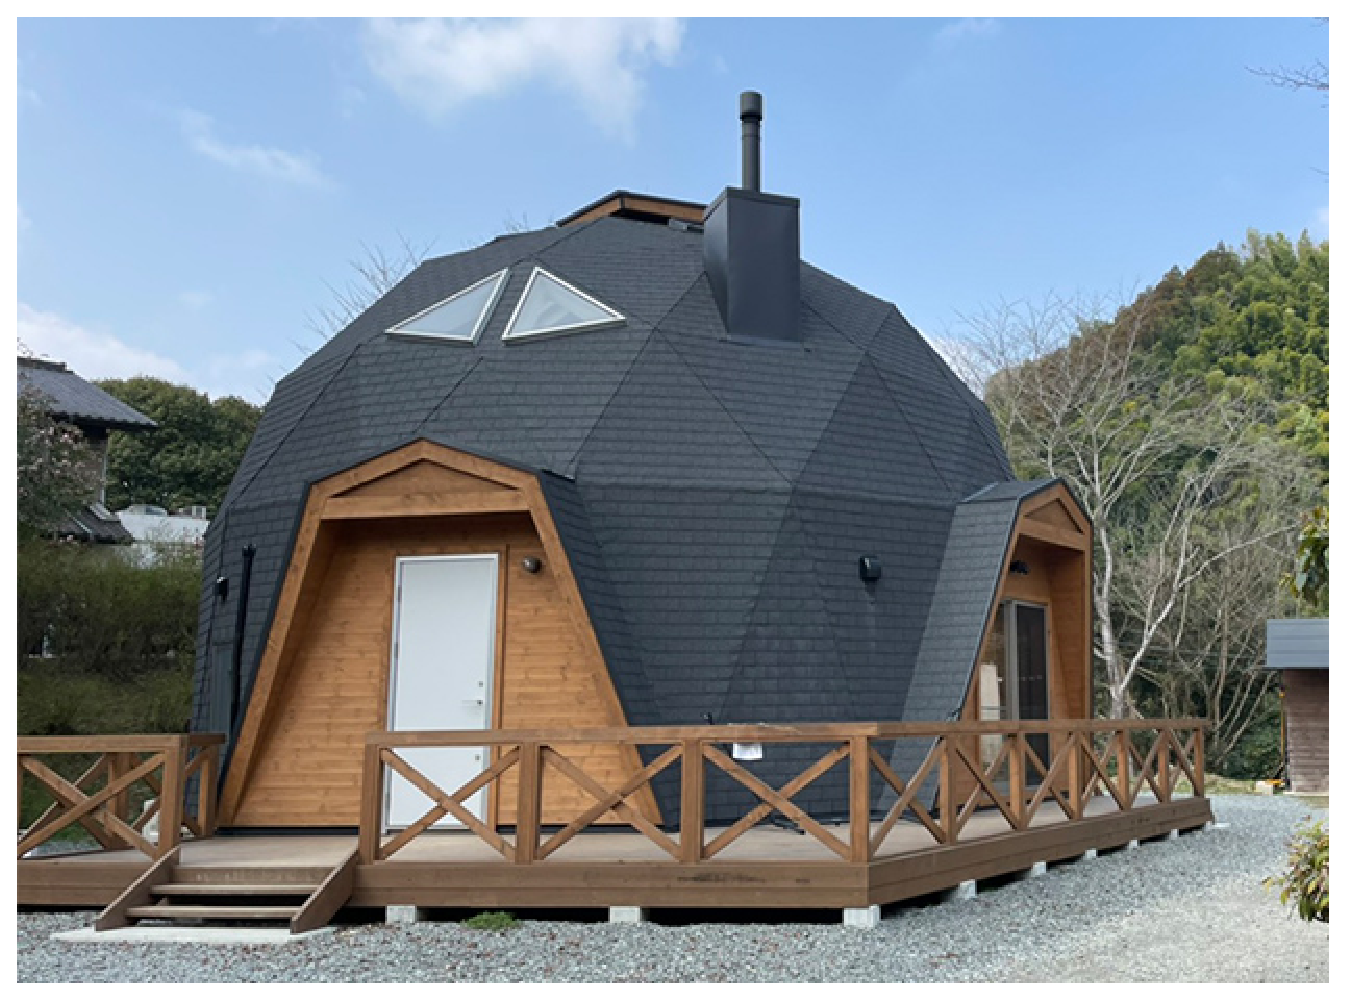
\includegraphics[width=\linewidth]{figures/domeHouse}
    \caption{ドームハウスの外観}
    \label{fig:domeHouse}
  \end{subfigure}
  \hfill
  \begin{subfigure}{0.4\linewidth}
    \centering
    
\includegraphics[width=\linewidth]{figures/inside}
    \caption{ドームハウスの内観}
    \label{fig:inside}
  \end{subfigure}
  \caption{ドームハウスの環境}
  \label{fig:Device1}
\end{figure}



\FloatBarrier

\subsection{電車内における測定環境}

本測定は,実際の公共交通機関における空気環境を評価することを目的として,走行中の電車内において実施した。測定対象は,JR九州 鹿児島本線を走行する一般的な通勤型車両とし,香椎駅から鳥栖駅までの区間において測定を行った。測定に使用した車両は813系電車であり,車内はロングシート構成を基本とし,各車両には複数のドアおよび窓が設置されている。通勤時間帯に運行される車両であるため,乗客の乗降や車内の人員密度の変化が生じやすい環境である。

図\ref{fig:Train Car Environment}に,測定を行った電車内の概略図を示す。図中の緑色部分はドア位置,青色部分は窓位置を表している。本研究では,車内における位置の違いが二酸化炭素(CO$_2$)濃度に与える影響を評価するため,異なる2箇所に携帯型測定デバイスを装着した人を配置した。

CS1は,ドアから離れた座席位置に着席した被験者の腰部に装着し,乗客の乗降や外気流入の影響を比較的受けにくい位置におけるCO$_2$濃度を測定した。一方,CS2はドア付近の座席に着席した被験者の腰部に装着し,乗客の乗降やドア開閉による外気流入の影響を受けやすい位置でのCO$_2$濃度を測定した。いずれの測定においても,被験者は着席状態を維持しており,測定デバイスは腰部に装着することで,歩行や立位による影響を排除した条件で測定を行った。

\begin{figure}[H]
\centering
\includegraphics[width=0.5\linewidth, angle=-90]{./figures/train2}
\caption{
電車内の環境
}
\label{fig:Train Car Environment}
\end{figure}

\section{測定方法}

\subsection{センサの基礎特性確認}

実環境における測定に先立ち,使用するCO$_2$測定デバイスが,CO$_2$測定機器の選定ガイドラインに示される基本的な応答特性を有しているかを確認するため,アルコールおよび呼気に対する反応を評価する基礎的な測定を実施した。本測定では,12時に測定を開始し,30秒間隔でCO$_2$濃度を記録した。測定開始から20分後に,アルコールを入れたコップおよびアルコールを浸したティッシュを測定デバイス近傍に設置し,約10分間静置した。その後,測定開始から40分後に,測定デバイスに向けて1分間連続して呼気を吹きかけた。本測定の結果および評価については,次章において測定結果と併せて示す。

\subsection{据え置き型センサとの比較測定方法}

据え置き型CO$_2$センサと携帯型CO$_2$測定デバイスの測定値の整合性を確認するため,両センサを同一環境下に設置し,CO$_2$濃度の測定を行った。測定は13時30分から24時30分まで実施し,両センサともに5分間隔でCO$_2$濃度を記録した。本測定の結果および評価については,次章において示す。

\subsection{赤村ドームハウスにおける測定方法}

ドームハウス内における CO$_2$ 濃度分布および換気状態を把握するため,据え置き型 CO$_2$ 測定器と,本研究で試作した小型 CO$_2$ 測定デバイスを用いた測定を行った。本測定では,ドームハウス内部の高さ方向に着目し,床付近から天井付近にかけて CO$_2$ 濃度がどのように変化するかを評価することを目的とした。はじめに,先行研究で使用された据え置き型 CO$_2$ 測定器を用いて測定を行った。据え置き型測定器は合計 35 台使用し,螺旋階段および 2 階部分に設置された棚を含め,床面付近から天井付近までの高さ方向に配置した。各測定器には EXAKA1 から EXAKA35 の識別子を付与し,EXAKA1 を最下部,EXAKA35 を最上部とした。測定は同一時間帯に実施し,各測定器から得られた CO$_2$ 濃度データを用いて,ドームハウス内における高さ方向の CO$_2$ 濃度分布を把握した。

次に,据え置き型測定器による測定結果を基準として,本研究で試作した小型 CO$_2$ 測定デバイスによる測定を行った。本測定では,多数のセンサを同時に設置する方法ではなく,利用者が携帯型デバイスを用いて任意の位置で測定を行う状況を想定し,小型 CO$_2$ 測定デバイスを携帯した状態で,ドームハウス内の異なる高さ位置において逐次的に CO$_2$ 濃度を測定した。比較測定の手順として,小型 CO$_2$ 測定デバイスを各据え置き型測定器の直近に配置し,同一高さ・同一空間における CO$_2$ 濃度を測定した。測定終了後,小型測定デバイスを一段上の設置位置へ移動させ,同様の測定を繰り返した。この操作を EXAKA1 から EXAKA35 までの全ての据え置き型測定器に対して順に実施し,合計 35 箇所における比較測定を行った。
測定時には,小型 CO$_2$ 測定デバイスと据え置き型 CO$_2$ 測定器が可能な限り近接するよう配置し,同一高さ・同一環境条件における CO$_2$ 濃度を測定できるよう配慮した。小型測定デバイスによる測定は,各高さ位置において測定ボタンを操作することで実施した。

\begin{figure}[htbp]
  \centering
  \begin{subfigure}{0.45\linewidth}
    \centering
    \includegraphics[width=\linewidth,angle=-90]{figures/akamurakaidan}
    \caption{階段}
    \label{fig:Device0}
  \end{subfigure}
  \hfill
  \begin{subfigure}{0.45\linewidth}
    \centering
    \includegraphics[width=\linewidth]{figures/akamura2kai}
    \caption{階段の上部}
    \label{fig:Finishing machine}
  \end{subfigure}
  \caption{プロトタイプおよび測定機器1の外観}
  \label{fig:Device1}
\end{figure}

\FloatBarrier

\subsection{電車内における測定方法}

測定は,JR九州 鹿児島本線において,香椎駅20時35分発の下り普通列車(813系)に乗車して実施した。本測定では,一定時間間隔による連続測定ではなく,各駅停車時におけるドア開閉の前後に着目した測定方法を採用した。具体的には,各駅においてドアが開く直前およびドアが閉まった直後のタイミングで携帯型CO$_2$測定デバイスによる測定を行った。これにより,乗客の乗降および外気流入が車内のCO$_2$濃度に与える影響を評価した。

図\ref{fig:kosimae}に,電車内測定時における携帯型センサの装着位置を示す。測定中は,CS1およびCS2のいずれにおいても,被験者は着席状態を維持し,測定デバイスは被験者の腰部に装着した状態で測定を行った。

\begin{figure}[H]
\centering
\includegraphics[width=0.5\linewidth, angle=-90]{./figures/kosimae}
\caption{
電車内測定時の携帯型センサの位置
}
\label{fig:kosimae}
\end{figure}





\section{評価方法}
本研究で実施した各測定により得られた結果については,赤村ドームハウスおよび電車内における測定結果に基づき,従来の据え置き型CO$_2$測定器との比較や,測定値の時間変化の傾向に着目して評価を行う。また,省電力性能については,バッテリ駆動時の連続稼働時間を指標として評価する。評価の詳細は次章において測定結果と併せて示す。

